\let\negmedspace\undefined
\let\negthickspace\undefined
\documentclass[journal]{IEEEtran}
\usepackage[a5paper, margin=10mm, onecolumn]{geometry}
%\usepackage{lmodern} % Ensure lmodern is loaded for pdflatex
\usepackage{tfrupee} % Include tfrupee package

\setlength{\headheight}{1cm} % Set the height of the header box
\setlength{\headsep}{0mm}     % Set the distance between the header box and the top of the text

\usepackage{gvv-book}
\usepackage{gvv}
\usepackage{cite}
\usepackage{amsmath,amssymb,amsfonts,amsthm}
\usepackage{algorithmic}
\usepackage{graphicx}
\usepackage{textcomp}
\usepackage{xcolor}
\usepackage{txfonts}
\usepackage{listings}
\usepackage{enumitem}
\usepackage{mathtools}
\usepackage{gensymb}
\usepackage{comment}
\usepackage[breaklinks=true]{hyperref}
\usepackage{tkz-euclide}
\usepackage{listings}                                     
\def\inputGnumericTable{}                                 
\usepackage[utf8]{inputenc}                                
\usepackage{color}                                            
\usepackage{array}                                            
\usepackage{longtable}                                       
\usepackage{calc}                                             
\usepackage{multirow}                                         
\usepackage{hhline}                                           
\usepackage{ifthen}                                           
\usepackage{lscape}
\renewcommand{\thefigure}{\theenumi}
\renewcommand{\thetable}{\theenumi}
\setlength{\intextsep}{10pt} % Space between text and floats

\numberwithin{equation}{enumi}
\numberwithin{figure}{enumi}
\renewcommand{\thetable}{\theenumi}

% Marks the beginning of the document
\begin{document}
\bibliographystyle{IEEEtran}

\title{Question-9.4.19}
\author{EE24BTECH11048-NITHIN.K} 
%\maketitle
%\newpage
%\bigskip
{\let\newpage\relax\maketitle}
\textbf{Question:} \\
  The volume of spherical balloon being inflated changes at a constant rate. If initially its radius is 3 units and after 3 seconds it is 6 units. Find the radius of balloon after t seconds. \\ 

\textbf{Solution:} \\
$r_0$: Initial radius of the sphere = 3 units. \\
$r_3$: Radius of the sphere at 3 seconds = 6 units. \\
t: The time after which the radius $r_t$ is to be found. \\
K: rate of change in volume \\
  It is given that the rate of change in volume is constant hence \\
  \begin{align}
	  \frac{dV}{dt} = K
  \end{align}
  \begin{align}
	  \frac{dV}{dt} = \frac{V_3 - V_0}{3-0}
  \end{align}
  \begin{align}
	  K = \frac{1}{3} \times \brak{\frac{4\pi {r_3}^3}{3} - \frac{4\pi {r_0}^3}{3}} = 84\pi
  \end{align}
  \begin{align}
	  \frac{dV}{dt} = K = 84\pi
  \end{align}
  \begin{align}
	  \frac{V_t - V_0}{t-0} = 84\pi
  \end{align}
  \begin{align}
	  V_t = V_0 + 84\pi t
  \end{align}
  \begin{align}
	  \frac{4\pi {r_t}^3}{3} = \frac{4\pi {r_0}^3}{3} + 84\pi t
  \end{align}
  \begin{align}
	  r_t = \brak{{r_0}^3 + 63t}^{\frac{1}{3}}
  \end{align}
Substituting equation 0.3 in 0.1
  \begin{align}
	  \frac{dV}{dt} = 84\pi
  \end{align}
  \begin{align}
	  \frac{4\pi r^2dr}{dt} = 84\pi
  \end{align}
  \begin{align}
	  \frac{dr}{dt} = \frac{21}{r^2}
  \end{align}
  \begin{align}
	  \frac{dy}{dx} = \frac{21}{y^2}                      
  \end{align}
  \begin{align}
          \frac{y_{n+1} - y_n}{dx} = \frac{21}{{y_n}^2}
  \end{align}
  \begin{align}
          y_{n+1} = \frac{21dx}{{y_n}^2} + y_n
  \end{align}

\begin{figure}[H]
    \centering
    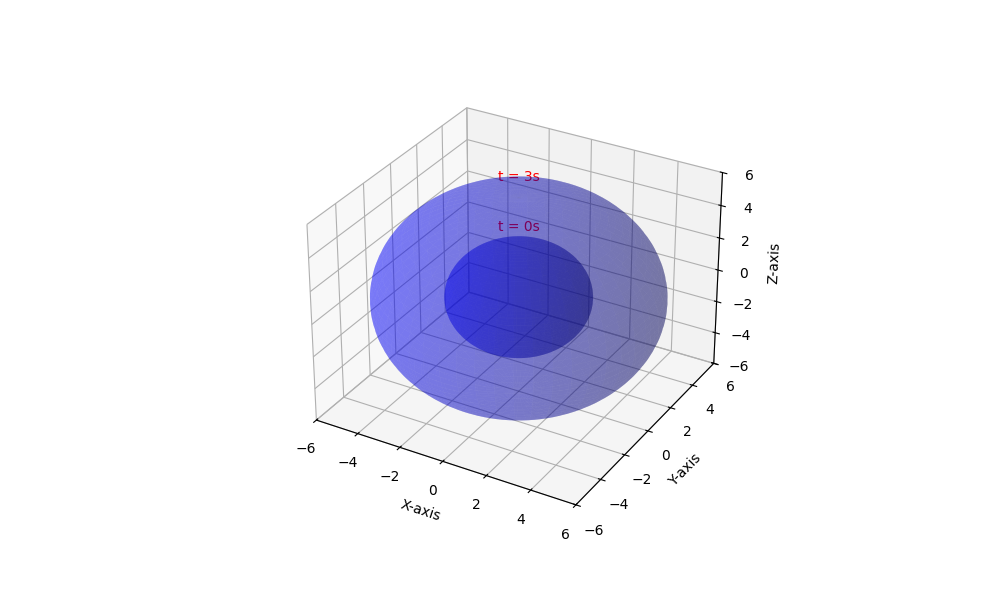
\includegraphics[width=\textwidth]{figs/growing_sphere.png}
    \caption{Sphere growing over time.}
\end{figure}

\begin{figure}[H]
    \centering
    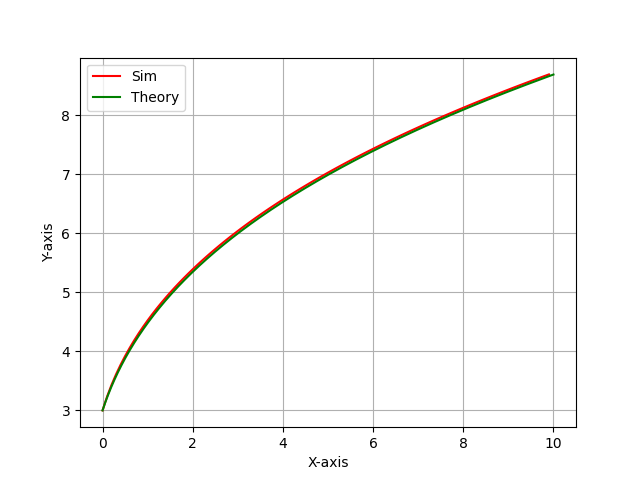
\includegraphics[width=0.8\textwidth]{figs/fig.png}
    \caption{Simulation VS Theoretical Plot.}
\end{figure}



\end{document}
